\documentclass{beamer}
\usepackage{beamerthemeshadow}
\usepackage{graphicx}
\usepackage{color}
\usepackage[utf8]{inputenc}
\usepackage{hyperref}
\usepackage[english,serbian]{babel}
\usepackage[flushleft]{threeparttable}
\definecolor{beamer@darkblue}{rgb}{0, 0, 232}
\setbeamercolor{structure}{fg=beamer@darkblue}

\def\d{{\fontencoding{T1}\selectfont\dj}}
\def\D{{\fontencoding{T1}\selectfont\DJ}}


\title{Tehničko i naučno pisanje}
\subtitle{-- Poređenje različitih vrsta prenosa podataka na mobilnom telefonu --}
\author{Vojin Knežević, Andrija Soković, Nenad Pešić i Vukašin Cupara}
\institute{Matematički fakultet\\Univerzitet u Beogradu}
\date{
	\footnotesize{Beograd, 2022.}	
}

\begin{document}
\begin{frame}
	\thispagestyle{empty}
	\titlepage
\end{frame}

\addtocounter{framenumber}{-1}

\begin{frame}{Literatura}
	\begin{itemize}
		\item Structure of Wireless Ad Hoc Network (\url{ResearchGate.net})
        \item What Is GSM (Global System for Mobile Communications) Meaning, Working, Architecture, and Applications (\url{spiseworks.com})
        \item Near-field communication (NFC) (\url{techtarget.com})
        \item Računarske mreže (\url{bpa.edu.rs})
        \item Wireless Networks (\url{ccontrols.net})
		
	\end{itemize}
\end{frame}

\begin{frame}
	\frametitle{Pregled} 
	\tableofcontents[hidesubsections] 
\end{frame}

\section{Uvod}

\begin{frame}{Uvod}
\begin{itemize}
\item Razmena podataka - proces pouzdanog slanja podataka između 2 ili više učesnika u komuniciranju.\\
\item Računarske mreže dele se na:
\begin{enumerate}
    \item Broadcast mreže (emisija svima)
    \item Point to point (između 2 računara)
\end{enumerate}
\item Podela mreže prema vrsti medijuma:
\begin{enumerate}
    \item Žične (fizički medijum - bakarni kabl)
    \item Bežične (medijum je etar, vazduh)
\end{enumerate}
\end{itemize}
	
\end{frame}

\section{Bežične mreže}
\begin{frame}{Bežične mreže}

\begin{itemize}
\item Kategorije: Ad-hoc, Celularne(ćelijske), Point to point;
\begin{enumerate}
    \item Ad-hoc - direktno uspostavljanje komunikacije; čvorovi
    \item Ćelijske mreže - nemogućnost direktne komunikacije; preko pristupnih stanica 
    \item Point to point - komunikacija tačno dva uređaja; bez dodatne infrastrukture
\end{enumerate}
\item Bezbednost;
\end{itemize}

\begin{figure}[ht!]
\begin{center}
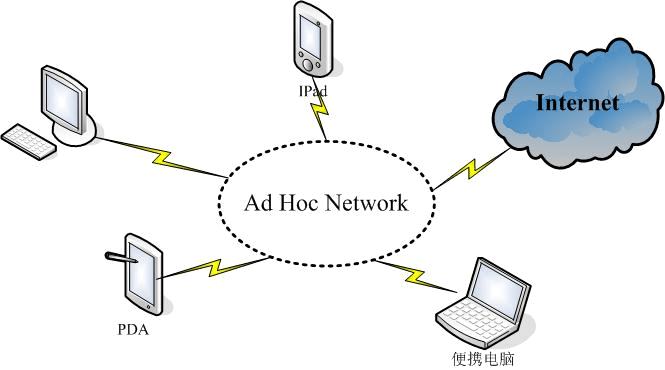
\includegraphics[scale=0.25]{AdHoc.png}
\end{center}
\caption{Ad-Hoc}
\label{fig:adhoc}
\end{figure}
\end{frame} 

\section{Vrste bežičnih mreža koje koriste mobilni telefoni}
\begin{frame}{Vrste bežičnih mreža koje koriste mobilni telefoni}
\begin{itemize}
\item Podela prema nameni i području koje pokrivaju:
\begin{itemize}
    \item WWAN (Wireless Wide Area Network): \textbf{GSM}, \textbf{LTE} i \textbf{CDPD}
    \item WLAN (Wireless Local Area Network): \textbf{Wi-Fi} i \textbf{Li-Fi}
    \item WPAN (Wireless Personal Area Network): \textbf{Bluetooth}, \textbf{NFC} i \textbf{Infrared}
\end{itemize}
\item \textbf{GSM}: Prenos govora, prenos podataka(9,6 Kb/s) i slanje SMS poruka.
\item \textbf{LTE}: Manja cena po bitu i veći aspekt servisa.
\end{itemize}

\begin{figure}[!ht]
\begin{center}
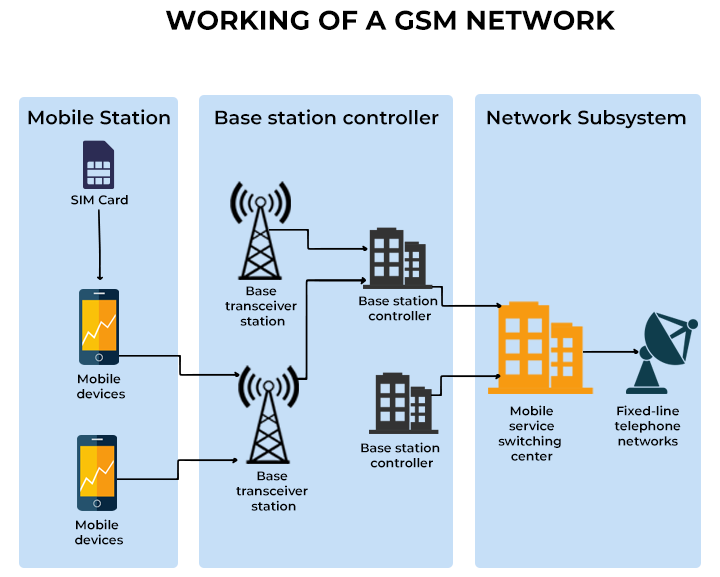
\includegraphics[scale=0.15]{GSM.png}
\end{center}
\caption{GSM mreža}
\label{fig:GSM}
\end{figure}
    
\end{frame} 
\begin{frame}{Vrste bežičnih mreža koje koriste mobilni telefoni}
\begin{itemize}
    \item \textbf{Wi-Fi}
        \begin{enumerate}
            \item Domet: do 70m u zatvorenom i 250m na otvorenom prostoru;
            \item Brzina: 54Mbps – 3.5Gbps (zavisi od standarda);
        \end{enumerate}
    \item \textbf{Li-Fi}
        \begin{enumerate}
            \item Domet: oko 10m;
            \item Brzina: do 1Gbps;
        \end{enumerate} 
    \item \textbf{Bluetooth}
        \begin{enumerate}
            \item Brzina: od 700Kbps do 3Mbps;
            \item Domet: do 10m;
        \end{enumerate}
    \item \textbf{Infrared}
        \begin{enumerate}
            \item Neophodna je optička vidljivost (usmeren ili difuzan mod);
            \item Domet: oko 3m;
        \end{enumerate}
    \item \textbf{NFC}
        \begin{enumerate}
            \item Domet: do 10cm;
            \item Nema potrebe za napajanjem prilikom korišćenja osnovnih funkcija (slušanje i odgovaranje na poruke);
        \end{enumerate}
\end{itemize}
\end{frame}
\section{Pregled glavnih karakteristika različitih vrsta mreža}
\begin{frame}{Pregled glavnih karakteristika različitih vrsta mreža}
    \begin{center}
\scalebox{0.65}{%
    \begin{tabular}{|c|c|c|c|} 
      \hline
      \textbf{Vrsta bežičnog prenosa} & \textbf{Brzina prenosa (u Mbps)} & \textbf{Frekvencija (u MHz)} & \textbf{Domet (u metrima)} \\
      \hline
      GSM & 0.0096 & 890-960 & do 40000 \\
      LTE & 50/100 & 1900-2100 & do 8000 \\
      Bluetooth & 0.7-3 & 2400 & 10 \\
      Infrared & 10-16 & 3 x $10^{8}$ & 3 \\
      NFC & 0.4 & 13.56 & 0.1 \\
      Wi-Fi & do 3500 & 2400/5000 & 70 \\
      Li-Fi & do 1000 & 2 x $10^{8}$ & 10 \\
      \hline
    \end{tabular}
}
  \end{center}
\end{frame} 

\section{Zaključak}
\begin{frame}{Zaključak}
	\begin{itemize}
	    \item Veoma je očigledno da prenos podataka na modernim telefonima uopšte nije jedinstven ni jednoličan, stoga ne postoji ni jedna tehnologija koja bi mogla da zadovolji uopšteno sve potrebe, a da pritom ostane efikasna u svojoj komunikaciji.
        \item Različite tehnologije, osim sa tehničke strane realizacije komunikacije, korisnicima omogućavaju potpuno različita korisnička iskustva i omogućavaju nesmetanu upotrebu mobilnih telefona u svakodnevnom životu.
	\end{itemize}
\end{frame}

\end{document}